%!TEX root = ../thesis.tex
%*******************************************************************************
%****************************** Fourth Chapter *********************************
%*******************************************************************************

\chapter{Benchmark}
\label{chap:benchmark}
\ifpdf
    \graphicspath{{Chapter4/Figs/Raster/}{Chapter4/Figs/PDF/}{Chapter4/Figs/}}
\else
    \graphicspath{{Chapter4/Figs/Vector/}{Chapter4/Figs/}}
\fi

\topic{Il faut un benchmark solide pour comparer les méthodes}

\section{Constitution du benchmark} % (fold)
\label{sec:constitution_du_benchmark}

\content{Weak baselines, too many (too complex or specific) objective functions and other problems in presenting ML results.}

\victor{Ce que j'essaie de faire c'est mettre un peu d'ordre. Donc je doit décrire les métriques utilisée par les autres papier. Décrire ce que je veux ranger}


\section{Toy datasets} % (fold)
\label{sec:toy_datasets}




\subsection{Apple and pears} % (fold)
\label{sub:apple_and_pears}

Let's start with a toy problem and make it gradually more complex.
The study is about finding the proportion $\mu$ of apples and pears in a bag.
The only information available is the total number of fruits in the bag and the weight of each individual fruit.
Apples and pears weights are normally distributed and slightly different.
The dataset is a set of real values $D = \{ x_i \in \RR \} $

From the average weight of the fruits in the bag a linear regression is enough to find the link between $D$ and the parameter of interest $\mu$.
The model can be trained if enough bags in which the proportion is known is available for training.
This simplicity is wanted to test the method.

Since the weight of a fruit is stochastic, two bags of fruits with the same number of apples and pears may have a different average weight.
Leading to some uncertainty in the predicted proportion that must be reported.






\subsection{Toy 1D} % (fold)
\label{sub:toy_1d}

The toy that will interest us here is a mixture of 2 distributions with an observable $x \in \RR$.
A gamma that will represent the background process and a gaussian to represent the signal process.
\autoref{fig:minitoy_distrib} presents the data distribution for a 10,000 instances sampling.

The parameter of interest is the mixing coefficient of the 2 $y$ distributions.
The nuisance parameter $\alpha$ is a rescaling of the observable $x$.

Without nuisance parameter $\alpha$ the likelihood is :
$$
    p(x | y) = y \mathcal N(x|a, b) + (1-y) \Gamma(x|s, \theta)
$$

Including nuisance parameter $\alpha$ the likelihood becomes :
$$
    p(x | y, \alpha) = y \mathcal N(x|\alpha a, \alpha b) + (1-y) \Gamma(x|\alpha s, \theta)
$$

\begin{figure}[htb]
    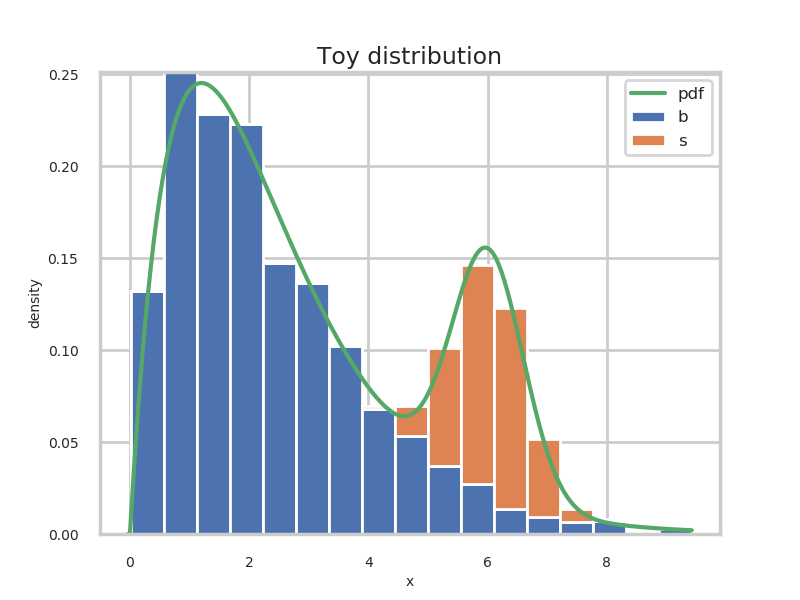
\includegraphics[width=\linewidth]{minitoy/distrib.png}
    \caption{Data distribution of the 1D toy}
    \label{fig:minitoy_distrib}
\end{figure}




\subsection{Toy 3D} % (fold)
\label{sub:toy_3d}

To get closer to the reality the toy example introduced in \cite{DECASTRO2019170inferno} is also included.
This toy is a mixture of 2 process named background and signal as usual.


For the backgrounds :
$$
f_b (x|r, \lambda) = \mathcal N \left ( (x_0, x_1) | (2+r, 0) 
\begin{bmatrix} 5 & 0 \\ 0 & 9 \end{bmatrix} \right ) Exp((x_2| \lambda)
$$


For the signals :
$$
f_s (x|r, \lambda) = \mathcal N \left ( (x_0, x_1) | (1, 1) 
\begin{bmatrix} 1 & 0 \\ 0 & 1 \end{bmatrix} \right ) Exp((x_2| 2)
$$

Leading to the likelihood :
$$
p(x | r, \lambda, \mu ) = (1-\mu) f_b(x|r, \lambda) + \mu f_s(x|r, \lambda)
$$

This toy is multi dimensional, more complex and includes 2 nuisance parameters.

\autoref{fig:s3d2_pairgrid} shows the distributions of a sampled dataset.

\begin{figure}[htb]
    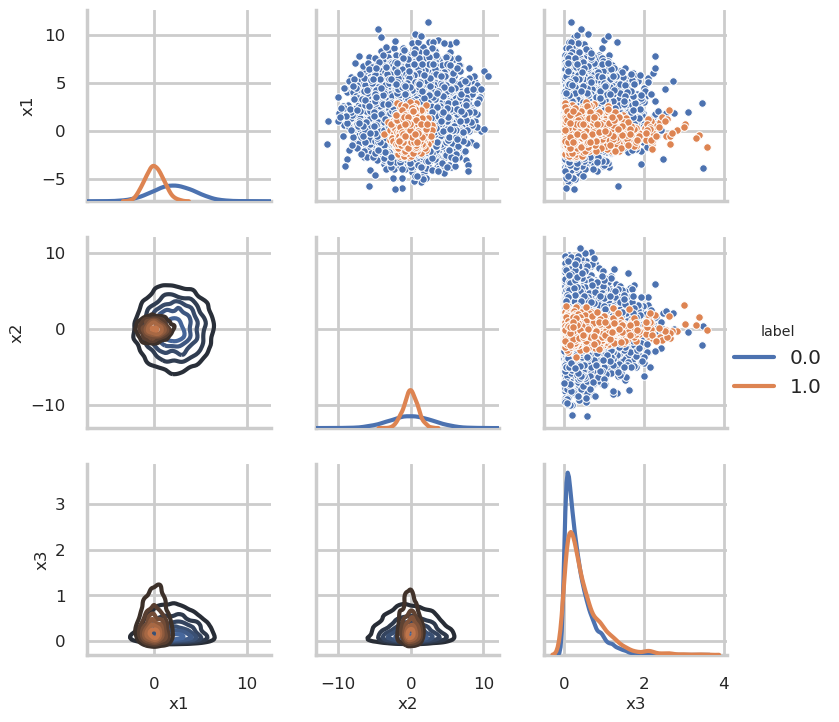
\includegraphics[width=\linewidth]{s3d2/pairgrid}
    \caption{Data distribution of the 3D toy}
    \label{fig:s3d2_pairgrid}
\end{figure}






\section{Higgs data} % (fold)
\label{sec:higgs_data}



\subsection{Simulation} % (fold)
\label{sub:simulation}

\content{Un peu de blabla sur Geant4 \needcite et à quel points ces simulations sont complexes.}
\content{importance weight}



\subsection{HiggsML challenge} % (fold)
\label{sub:higgsml_challenge}

\content{Petit rappel sur le challenge qui a permi à ces données d'exister et d'être publique !}
\content{détails : \#samples, \#features, etc}
\content{Perte de DER\_mass\_mmc ??}




\subsection{Nuisance parameters} % (fold)
\label{sub:nuisance_parameters}

\content{simulateur rapide}
\content{nuisance parameters}





\section{Best inference on toys} % (fold)
\label{sec:best_inference_on_toys}

The toy data does not suffer from intractable likelihood making it possible to compute the posterior probability using standard bayesian inference.
The computed posterior is the best possible inference and will be compared with the other methods that assumes the likelihood is intracteble.

\subsection{Computing the posterior} % (fold)
\label{sub:computing_the_posterior}

\victor{Trop de détail : à déplacer dans l'appendice A}

Computing the integral by hand can be tedious.
The simple method proposed allow to avoid it.

Start with a grid, fine enough, going through the possible values. $y_i, \alpha_j$.

From Bayes theorem : 
$$
    p(y_i, \alpha_j | x) = \frac{p(x|y_i, \alpha_j) p(y_i, \alpha_j)}{p(x)}
$$

The 2 following tensor can be computed from the simulator.
\begin{itemize}
  \item likelihood : $L_{ij} = p(x|y_i, \alpha_j)$
  \item prior : $K_{ij} = p(y_i, \alpha_j)$ 
\end{itemize}

giving the tensor $ R_{ij} = p(x|y_i, \alpha_j) p(y_i, \alpha_j) $ 
which after renormalization gives the posterior tensor $ T_{ij} = p(y_i, \alpha_j | x)$.

The marginal probabilities are computed from $T_{ij}$ :
\begin{itemize}
  \item $p(y_i | x) = \sum_j T_{ij} = Y_i$
  \item $p(\alpha_j | x) = \sum_i T_{ij} = A_j$
\end{itemize}

the neural network should compute : $p(y_i | x, \alpha_j) = \frac{p(y_i, \alpha_j | x)}{p(\alpha_j | x)} = \frac{T_{ij}}{A_j} = N_{ij}$

We then obtain the quantities we are interested in :
\begin{itemize}
  \item $ \VV(y|x) = \VV(y_i, Y_i) $
  \item $ \EE_{\alpha \sim p(\alpha|x)}[ \VV(y|x, \alpha) ] = \sum_j \VV(y|x, \alpha_j) p(\alpha_j | x) = \sum_j \VV_i(y_i, N_{ij}) A_j$
  \item $\EE_{\alpha \sim p(\alpha|x)} \left ((\EE [y|x, \alpha]  - \EE[y|x])^2\right ) = \VV(y|x) - \EE_{\alpha \sim p(\alpha|x)}[ \VV(y|x, \alpha) ] = \VV(y_i, Y_i) - \sum_j \VV_i(y_i, T_{ij}) A_j$
\end{itemize}


\subsubsection{Note 1}

For the computations it is necessary to remember that the tensors contain probabilities !
Meaning $<y|x>= \EE[y|x] = \sum_i y_i Y_i$ because $Y_i$ only contains probability densities, not values of $y$ !

Same applies for $\VV(y|x) = \sum_i y_i^2 Y_i - <y|x>^2 = \VV(y_i, Y_i)$


\subsubsection{Note 2}

For numerical stability it is best to work with log probabilities.

Indeed $x$ is a dataset so $p(x | y_i, \alpha_j) = \prod_k^N p(x_k | y_i, \alpha_j)$ for N big enough to obtain too small number to be stored in 64 bits.

It is smarter to compute : $\log p(x | y_i, \alpha_j) = \sum_k^N log p(x_k | y_i, \alpha_j) = \ell(x | y_i, \alpha_j)$
Then $\ell(y_i, \alpha_j| x) = \log p(x|y_i, \alpha_j) + \log p(y_i, \alpha_j)$

And renormalizing using a softmax :
$$ 
    T_{ij} = p(y_i, \alpha_j | x) = \frac{e^{\ell(y_i, \alpha_j| x)} }{\sum_{n,m} e^{\ell(y_n, \alpha_m| x)} }
$$


\subsubsection{Note 3}

If there is multiple nuisance parameters $\alpha$, $\beta$, etc the tensor are simply n-dimensional : $L_{ijk...}$, $T_{ijk...}$, $K_{ijk...}$, etc.
And all sums over $j$ become summs over $j,k, ...$ which is easily handle with broadcasting in modern numeric libraries.



\section{Evaluation metric} % (fold)
\label{sec:evaluation_metric}

\topic{The evaluation metric is the empirical mean squared error on the estimated parameters including variances}

Many methods to estimate the parameter of interest and its variance are available.
If changing the set of hyper parameter for the learning procedure is considered as changing the method then countless methods are to be evaluated.
Automating the measure of the performances of a proposed method is crucial to select the best method.
In this section is described a simple but general procedure to measure the performances of a given method.

The usual criterions to evaluate an estimator $\htheta$ are the bias, the variance and the mean squared error defined as follow :
\begin{equation}
  Bias(\htheta) = \EE[\htheta] - \thetas
\end{equation}
\begin{equation}
  Var(\htheta) = \EE[ (\htheta - \EE[\htheta])^2 ] = \EE[\htheta^2] - (\EE[\htheta])^2
\end{equation}
\begin{equation}
  MSE(\htheta) = \EE[(\htheta - \thetas)^2] = Var(\htheta) + [Bias(\htheta)]^2
\end{equation}

To evaluate these criterion we need to repeat the experiement $N$ times leading to many estimation of the parameters $\hmu^{(k)}$ and $\hshmu^{(k)}$.
Repeating the experiment can be done through cross-validation methods.


\subsection{Evaluation of the parameter of interest estimator} % (fold)
\label{sub:evaluation_of_the_parameter_of_interest_estimator}

First, let's focus on evaluating the estimator of the parameter of insterest $\hmu$.
The true value of $\mu$, noted $\mus$, is available during tests since it is an input of the simulator.

From the estimation of its expected value
\begin{equation}
  \EE[\hmu] \approx <\hmu^{(k)}>_k = \frac{1}{N} \sum_{k} \hmu^{(k)}
\end{equation}
it is possible to estimated the criterions

\begin{equation}
  Bias(\hmu) \approx <\hmu^{(k)}>_k - \mus
\end{equation}
\begin{equation}
  \label{eq:var_hmu}
  Var(\hmu) \approx <\hmu^{(k)} \times \hmu^{(k)}>_k - (<\hmu^{(k)}>_k)^2
\end{equation}
\begin{equation}
  MSE(\hmu) = Var(\hmu) + [Bias(\hmu)]^2
\end{equation}




\subsection{Evaluation of the variance estimator} % (fold)
\label{sub:evaluation_of_the_variance_estimator}

The evaluation of the variance estimator $\hshmu$ could be done in the same way if the true variance $Var(\hmu)$ can be computed.
If this is not the case an approximation is available using \autoref{eq:var_hmu}.

\begin{equation}
  Bias(\hshmu) \approx <\hshmu^{(k)}>_k - Var(\hmu)
\end{equation}
\begin{equation}
  Var(\hshmu) \approx <\hshmu^{(k)} \times \hshmu^{(k)}>_k - (<\hshmu^{(k)}>_k)^2
\end{equation}
\begin{equation}
  MSE(\hshmu) = Var(\hshmu) + [Bias(\hshmu)]^2
\end{equation}






\section{Details} % (fold)
\label{sec:details}



\subsection{Baselines} % (fold)
\label{sub:baselines}





\subsection{Neural network architectures} % (fold)
\label{sub:neural_network_architectures}

\content{How the architectures were chosen}




\subsection{Hyper-parameter search} % (fold)
\label{sub:hyper_parameter_search}

\content{Grid search on which HP}





\subsection{Cross validation} % (fold)
\label{sub:cross_validation}

\content{Shuffle split and seeding}







